\documentclass[UTF8]{article}
\usepackage{ctex,geometry,graphicx,float,makecell,rotating,multirow,diagbox}
\geometry{a4paper,scale=0.8}
\title{可信威胁与不可信威胁小论文}
\author{201850050\ 徐培宾}
\date{2022年5月22日}

\begin{document}
    \maketitle
    前段时间,世界首富马斯克在收购推特后发推文表示,下一步将要收购可口可乐公司,将几十年前从配料表中剔除的可卡因“重新“加入可乐中,此言一出,立即引起了众多媒体的关注,这样的威胁是否对\textbf{需要喝可乐}的顾客是否可信呢?

    首先我们根据问题总结一个博弈树。
    \begin{figure}[H]
      \centering
      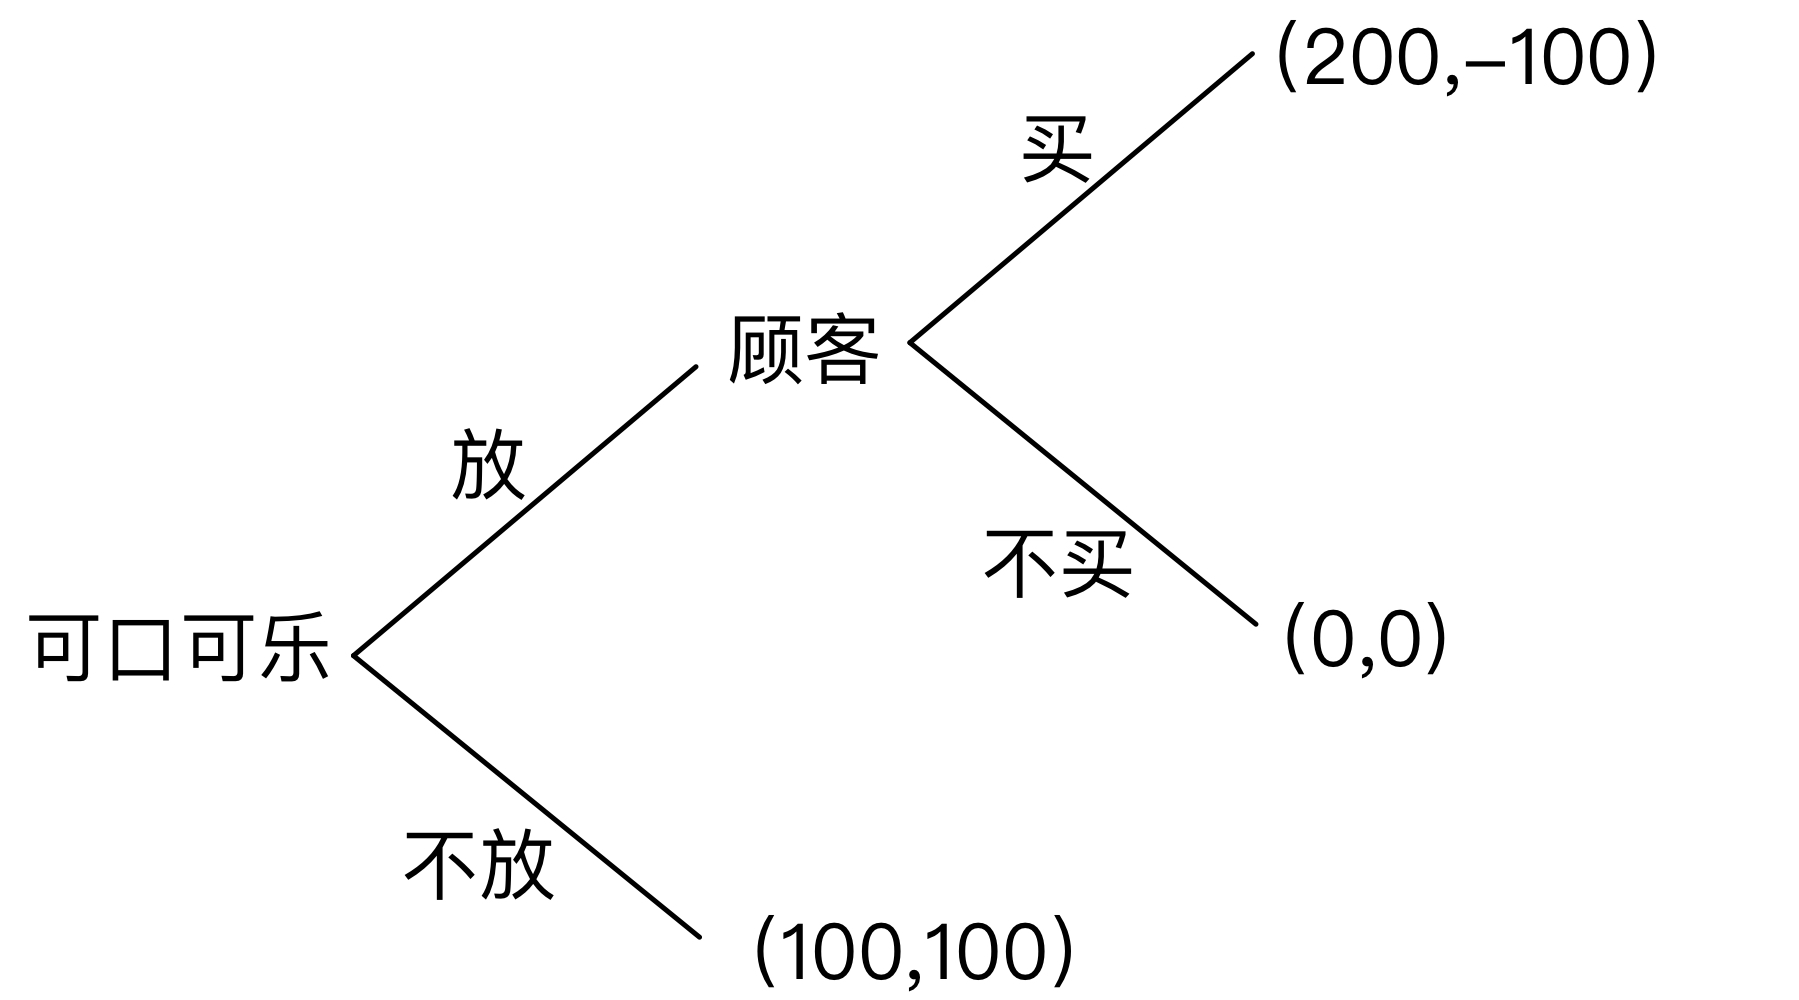
\includegraphics[width = 10cm]{cocacola.jpeg}
      \caption{向可口可乐中加入可卡因}
    \end{figure}
    \begin{itemize}
      \item 若可口可乐不放入可卡因,需要喝可乐的顾客仍然会购买,双方得益均为100。
      \item 若可口可乐添加可卡因,且顾客购买,可乐一定程度上会吸引顾客再次消费,得益变为200,但是顾客将会容易成瘾,对自身有害,得益变为-100。
      \item 若可口可乐添加可卡因,且顾客不购买,双方获益均为0。
    \end{itemize}
    
    可以发现,在加入可卡因之后,顾客会选择不买来获得更高的收益,而可口可乐的收益也变为0,比不加入可卡因时更低,因此其不会选择这样的策略,这是一种不可信威胁。

    但是,如果马斯克接下来收购百事可乐公司又会如何?

    事实上,当两家可乐巨头都被收购后,马斯克就将处于可乐产业的垄断地位,先前可以作为”加入可卡因的可口可乐“代替品的百事可乐也不复存在了。
    \begin{figure}[H]
      \centering
      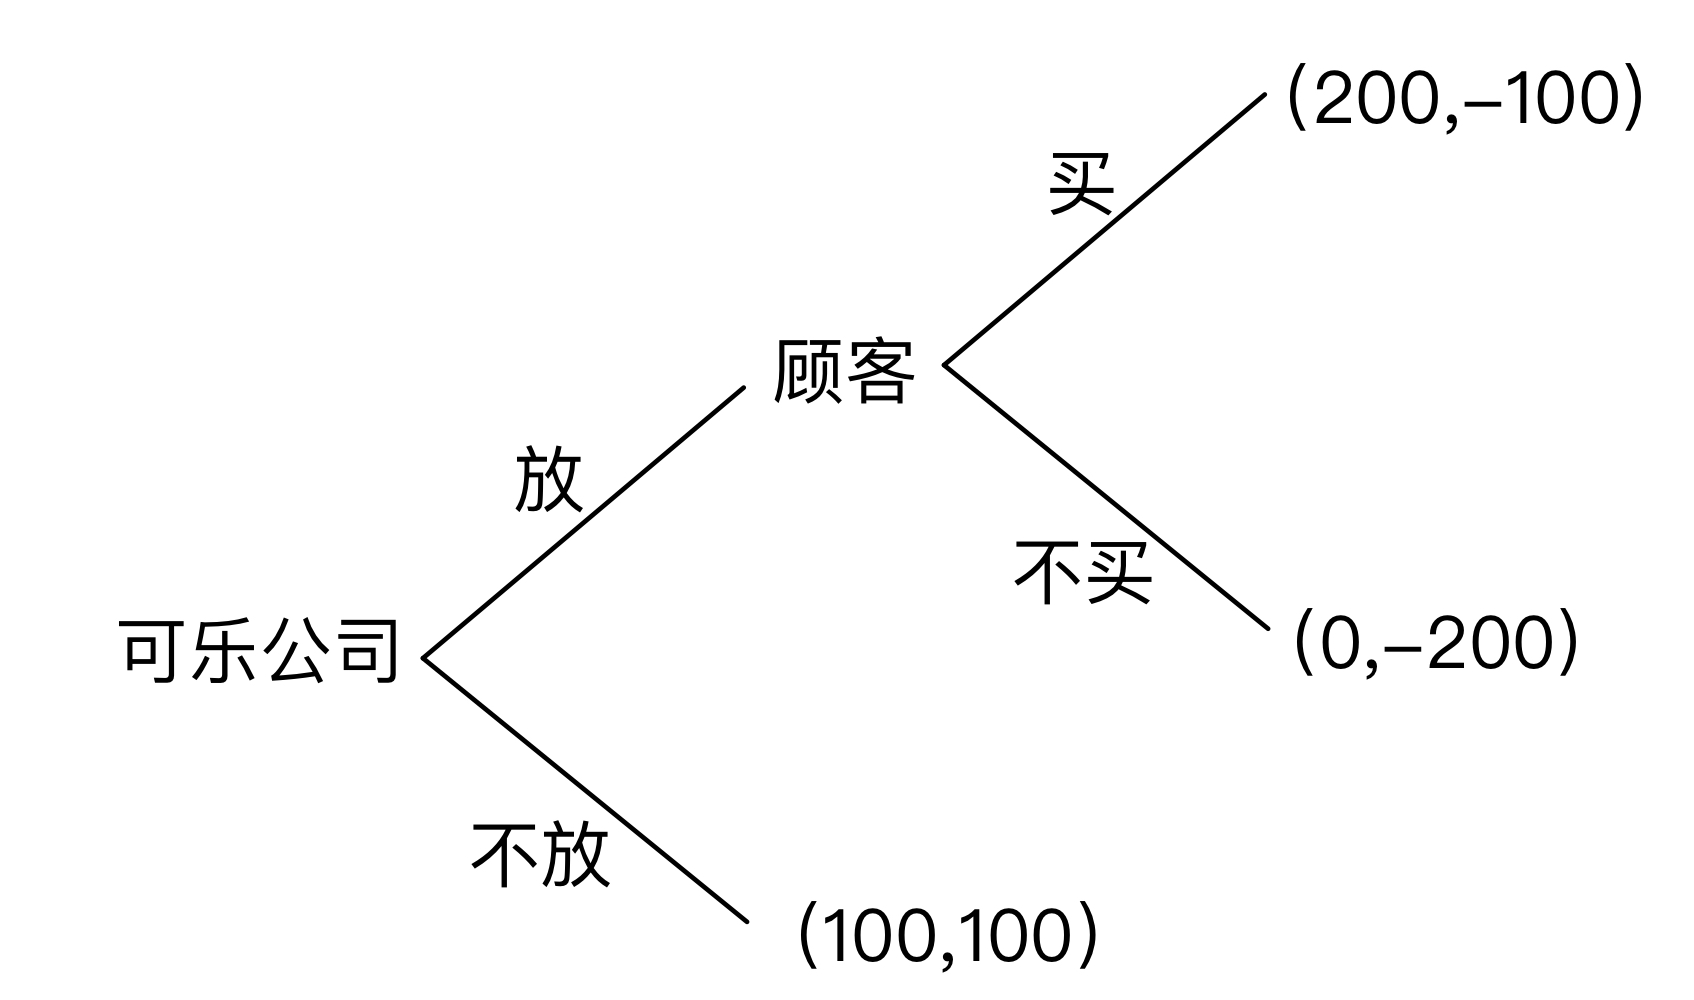
\includegraphics[width = 10cm]{cola.jpeg}
      \caption{向可乐中加入可卡因}
    \end{figure}
    \begin{itemize}
      \item 若可乐不放入可卡因,需要喝可乐的顾客仍然会购买,双方得益均为100。
      \item 若可乐添加可卡因,且顾客购买,可乐一定程度上会吸引顾客再次消费,得益变为200,但是顾客将会容易成瘾,对自身有害,得益变为-100。
      \item 若可乐添加可卡因,且顾客不购买,可乐公司得益为0,但是顾客无法从其他途径获得替代品(如之前的百事可乐),得益更低,为-200。
    \end{itemize}
    
    综上,不难看出,马斯克的这一番话是不可信威胁,但是如果其垄断了可乐产业,就应该当心,这样的言论可能会成真。
\end{document}